\documentclass[]{article}

% Imported Packages
%------------------------------------------------------------------------------
\usepackage{amssymb}
\usepackage{amstext}
\usepackage{amsthm}
\usepackage{amsmath}
\usepackage{enumerate}
\usepackage{fancyhdr}
\usepackage[margin=1in]{geometry}
\usepackage{graphicx}
\graphicspath{ {images/} }
\usepackage{extarrows}
\usepackage{setspace}
\usepackage[export]{adjustbox}
%------------------------------------------------------------------------------

% Header and Footer
%------------------------------------------------------------------------------
\pagestyle{plain}  
\renewcommand\headrulewidth{0.4pt}                                      
\renewcommand\footrulewidth{0.4pt}                                    
%------------------------------------------------------------------------------

% Title Details
%------------------------------------------------------------------------------
\title{Deliverable \#3 -- Detailed Design Document}
\author{SE 3A04: Software Design II -- Large System Design}
\author{Chen, Arthur \and Campbell, Christopher \and Endrizzi, Johnny \\ 
\and Coovert, Mitchell \and Gill, Surinder \and Dhadda, Terin}
\date{March 28, 2016}                              
%------------------------------------------------------------------------------

% Document
%------------------------------------------------------------------------------
\begin{document}

% Table of Contents
%------------------------------------------------------------------------------
\maketitle	
\newpage
\tableofcontents
\listoffigures
\listoftables
\newpage
%------------------------------------------------------------------------------

% Introduction
%------------------------------------------------------------------------------
\section{Introduction}
\label{sec:introduction}
The following section provides a brief overview of the entire document.

\subsection{Purpose}
\label{sub:purpose}
The purpose of this document is to lay out, in detail, the overall design of the "BEER'D" application. It will first give a description of the system and a general overview of what it is for, how it is expected to be used, and why it is being developed. It also contains more specific detail in terms of the states, sequences, and classes that will be implemented i the application. This document is intended primarily for the developers of the application, the professor, and the teaching assistants.

\subsection{System Description}
\label{sub:system_description}
The "BEER'D" system is a mobile application that aims to solve the question: "What beer is this?" This application is primarily being developed as a project for the third year Software Architecture class (course code SE 3A04) taught at McMaster University. A team of 6 students will design, develop, and create the application.\\
\\
The "BEER'D" application will take specific inputs from a user. Based on these inputs, varying "experts" will attempt to analyse and come up with their best prediction (based on data provided by publicly available API's) as to which beer the inputs may be identifying. The application will return and display a list of possible answers in a forum. Within this forum, users will also be able to share their answers on popular social media networks or find local stores which sell the beers referred to in the answers - based on their current location in an map.

\subsection{Overview}
\label{sub:overview}
The rest of the document is split up into three main sections:
\begin{enumerate}[-]
	\item The first section, State Charts for Controller Classes, will contain a state chart for each controller class for the application.
	\item The second section, Sequence Diagrams, will contain the sequence diagrams for each use case of the application (covered in the High Level Architectural Design document).
	\item The third and final section, Detailed Class Diagram, will contain the detailed class diagram for the application.
\end{enumerate}
%------------------------------------------------------------------------------




% State Charts for Controller Classes
%------------------------------------------------------------------------------
\newpage
\section{State Charts for Controller Classes}
\label{sec:state_charts_for_controller_classes}
The following section provides the state chart for each controller class for the application.
\begin{figure}[!htbp]
\includegraphics[scale=0.45, center]{state_diagram_1}
\caption{State Diagram Part 1 for the BEER'D Application}
\end{figure}
\begin{figure}[!htbp]
\includegraphics[scale=0.45, center]{state_diagram_2}
\caption{State Diagram Part 1 for the BEER'D Application}
\end{figure}
%------------------------------------------------------------------------------







% Sequence Diagrams
%------------------------------------------------------------------------------
\newpage
\section{Sequence Diagrams}
\label{sec:sequence_diagrams}
The following section provides the sequence diagram for each use case of the BEER'd application.
\begin{figure}[!htbp]
\includegraphics[scale=0.45]{sequence_diagram_1}
\caption{Sequence Diagram Part 1 for the BEER'D Application}
\end{figure}
\begin{figure}[!htbp]
\includegraphics[scale=0.45]{sequence_diagram_2}
\caption{Sequence Diagram Part 2 for the BEER'D Application}
\end{figure}
%------------------------------------------------------------------------------







% Detailed Class Diagram
%------------------------------------------------------------------------------
\newpage
\section{Detailed Class Diagram}
\label{sec:detailed_class_diagram}
The following section provides the detailed class diagram for the application.
\begin{figure}[!htbp]
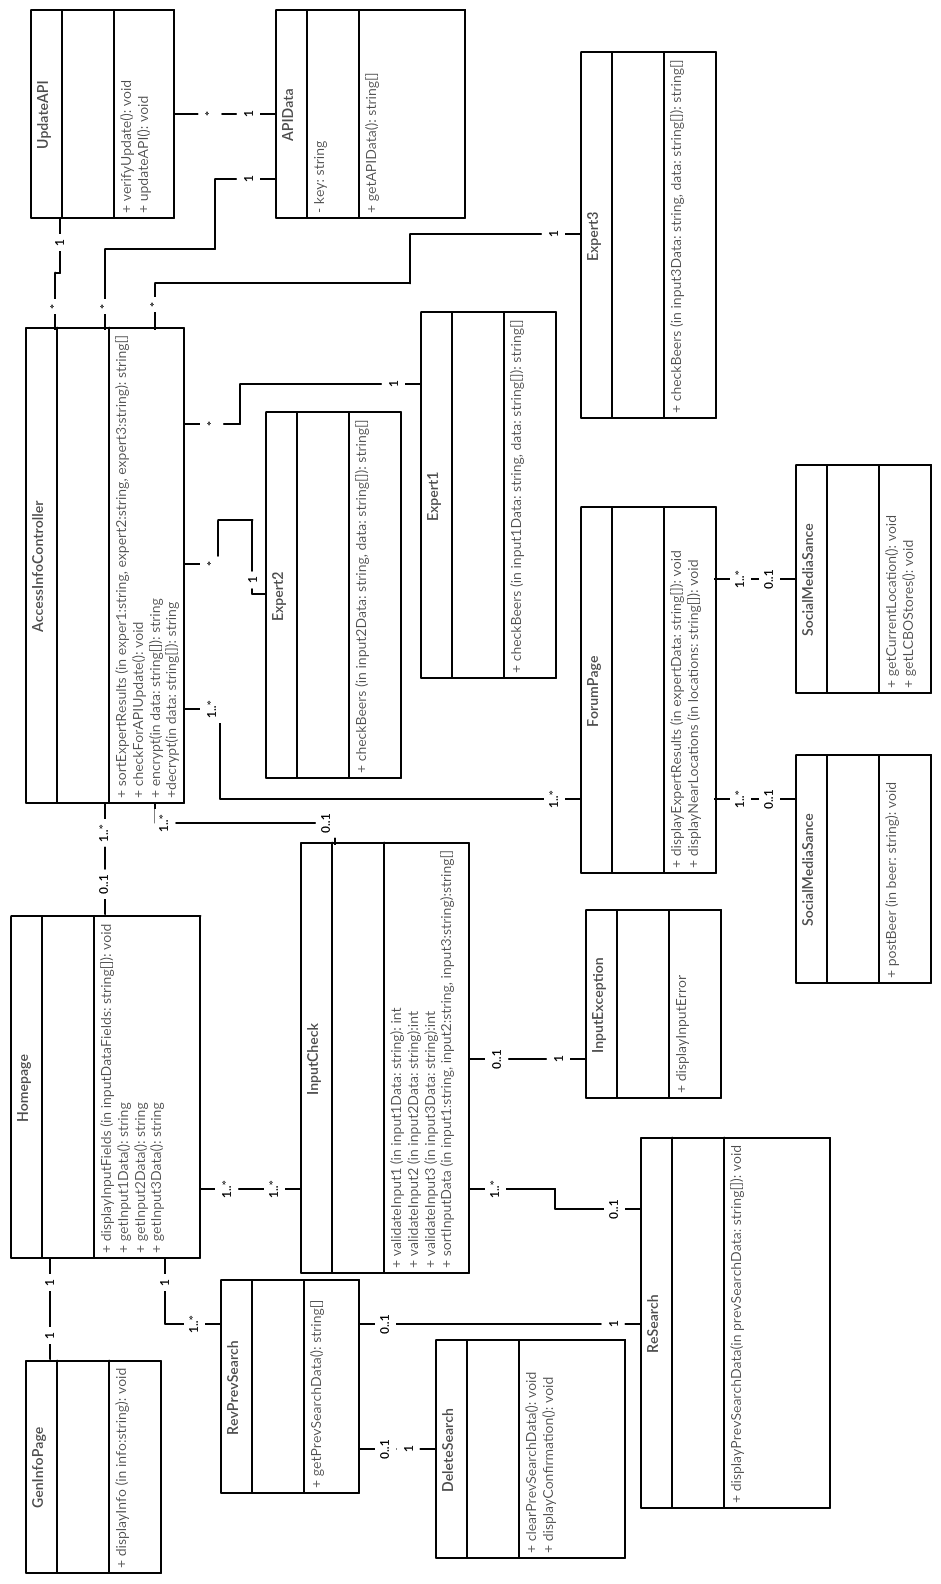
\includegraphics[scale=0.36, center]{detailedclass_diagram}
\caption{Detailed Class Diagram for the BEER'D Application}
\end{figure}
%------------------------------------------------------------------------------









% Division of Labour
%------------------------------------------------------------------------------
\newpage
\appendix
\section{Division of Labour}
\label{sec:division_of_labour}
\begin{table}[!htbp]
\centering
\begin{tabular}{|l|l|l|l|}
\hline
\multicolumn{1}{|c|}{\textbf{Team Member}} & \multicolumn{1}{c|}{\textbf{\begin{tabular}[c]{@{}c@{}}Student \\ Number\end{tabular}}} & \multicolumn{1}{c|}{\textbf{Contribution}} & \multicolumn{1}{c|}{\textbf{Signature}} \\ \hline
Arthur Chen & 1306616 & Sequence Diagram 2 &  \\ \hline
Christopher Campbell & 1143732 & Detailed Class Diagram &  \\ \hline
Johnny Endrizzi & 1310603 & State Diagram &  \\ \hline
Mitchell Coovert & 1306701 & State Diagram &  \\ \hline
Surinder Gill & 1308896 & Detailed Class Diagram, Composition &  \\ \hline
Terin Dhadda & 1312555 & Introduction, TOC, Sequence Diagram 1 &  \\ \hline
\end{tabular}
\caption{Contributions and Signatures of Team Members}
\end{table}
%------------------------------------------------------------------------------

\end{document}
%------------------------------------------------------------------------------
